\documentclass[11pt]{article}
\usepackage[a4paper,margin=1in]{geometry}
\usepackage{graphicx}
\usepackage{listings}
\usepackage{xcolor}
\usepackage{booktabs}
\usepackage{array}
\usepackage{hyperref}
\usepackage{parskip}
\hypersetup{colorlinks=true, linkcolor=black, urlcolor=blue}

\definecolor{codebg}{RGB}{245,245,245}
\lstdefinestyle{cppstyle}{
  language=C++,
  backgroundcolor=\color{codebg},
  basicstyle=\ttfamily\footnotesize,
  keywordstyle=\color{blue}\bfseries,
  commentstyle=\color{gray}\itshape,
  stringstyle=\color{teal},
  numbers=left,
  numberstyle=\tiny\color{gray},
  stepnumber=1,
  breaklines=true,
  frame=single,
  tabsize=2,
  showstringspaces=false
}
\lstdefinestyle{outstyle}{
  backgroundcolor=\color{codebg},
  basicstyle=\ttfamily\scriptsize,
  breaklines=true,
  frame=single,
  showstringspaces=false
}

\title{\vspace{-2cm}}
\date{}

\begin{document}
\begin{titlepage}
\centering
\vspace*{1cm}
{\large \textbf{Sri Sivasubramaniya Nadar College of Engineering}}\\
{\small (An Autonomous Institution, Affiliated to Anna University, Chennai)}\\
{\small Kalavakkam -- 603 110}\\[0.3cm]
{\small Department of Computer Science \& Engineering}\\[1.5cm]

\rule{\linewidth}{0.5mm}\\[0.4cm]
{\LARGE \textbf{Computer Networks Laboratory}}\\[0.3cm]
{\Large 1513 -- Computer Networks Lab}\\[0.4cm]
\rule{\linewidth}{0.5mm}\\[1.5cm]

{\huge \textbf{Assignment 9}}\\[0.4cm]
{\Large Simulation and Performance Analysis of TCP Congestion Control Algorithms using NS-3}\\[2cm]

\begin{center}
\begin{tabular}{ll}
\textbf{Name:} & Sundareswaran Rajaguru \\[0.2cm]
\textbf{Register Number:} & 3122247001048 \\[0.2cm]
\textbf{Year / Semester:} & III Year / V Semester \\[0.2cm]
\textbf{Course:} & 1513 Computer Networks Lab \\[0.2cm]
\textbf{Date of Submission:} & 21 June 2026 \\[0.2cm]
\end{tabular}
\end{center}

\vfill
\end{titlepage}

\section*{1. Objective}
To simulate an Intelligent Transportation System scenario in NS-3, where
vehicles send data through a roadside router to a traffic management server,
and to compare TCP Reno, TCP Cubic, and TCP BBR under congestion with respect
to throughput, delay, packet loss, fairness, and congestion window behaviour.

\section*{2. Topology}
\begin{center}
\begin{verbatim}
Vehicle0 --|
Vehicle1 --|
Vehicle2 --|---- Roadside Router ====Internet(bottleneck)==== Traffic Control Server
Vehicle3 --|
Vehicle4 --|
\end{verbatim}
\end{center}
Each vehicle-to-router access link is 5~Mbps/5~ms. The router-to-server link
(8~Mbps/20~ms) is the shared bottleneck representing the wider Internet path
from the roadside unit to the traffic control server. Five vehicles each run
one saturating TCP flow to the server; the congestion control algorithm used
by \emph{all} flows in a run is selected with \texttt{--tcpVariant}, so one
compiled program reproduces the Reno, Cubic, and BBR runs being compared.

\section*{3. Algorithm}
\begin{enumerate}
  \item Create 5 vehicle nodes, 1 roadside router node, and 1 server node;
        connect each vehicle to the router with a point-to-point access link,
        and the router to the server with the bottleneck link.
  \item Install the Internet stack on all nodes, assign one \texttt{/24}
        subnet per link, and populate global routing tables.
  \item Set \texttt{ns3::TcpL4Protocol::SocketType} to
        \texttt{TcpNewReno}, \texttt{TcpCubic}, or \texttt{TcpBbr} depending
        on \texttt{--tcpVariant} (TCP pacing is enabled globally, which BBR
        needs to behave correctly).
  \item Start one \texttt{BulkSendHelper} (continuous) TCP flow per vehicle to
        a distinct port on a \texttt{PacketSink} on the server, staggered by
        0.1~s each so the five flows don't start in perfect lock-step.
  \item Connect a trace callback on each vehicle's
        \texttt{TcpL4Protocol/SocketList/0/CongestionWindow} shortly after
        its flow starts, logging (time, cwnd) to a per-variant file.
  \item Install \texttt{FlowMonitor} on all nodes; run for 20~s; read back
        per-flow throughput, average delay, and packet loss, and compute
        Jain's Fairness Index across the five flows' throughputs.
\end{enumerate}

\section*{4. Code}
\subsection*{4.1 ass9.cc}
\lstinputlisting[style=cppstyle]{ns-3-work/scratch/ass9.cc}

\section*{5. Output}
\lstinputlisting[style=outstyle]{output.txt}

\section*{6. Congestion Window Behaviour}
\begin{center}
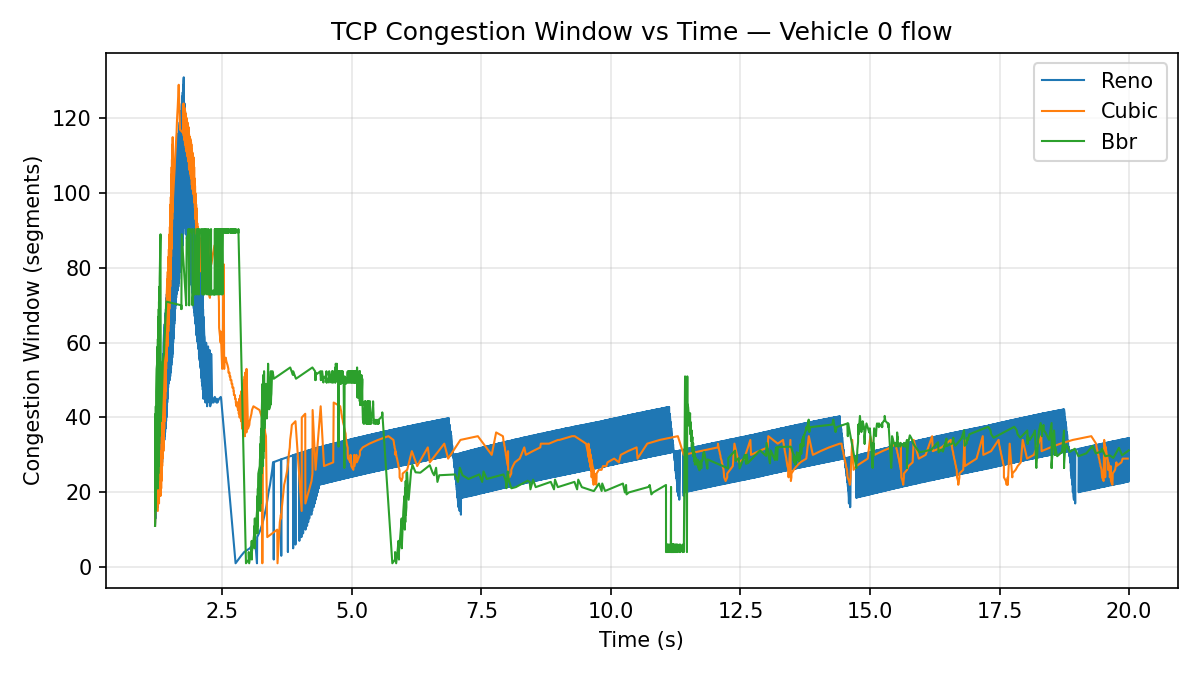
\includegraphics[width=0.85\textwidth]{screenshots/cwnd_comparison.png}
\end{center}
Reno shows the classic linear-growth/halve-on-loss sawtooth. Cubic grows more
aggressively along a concave curve and reaches a noticeably higher peak
window before backing off, since its window growth is a cubic function of
time since the last loss rather than a fixed additive increase. BBR's window
does not follow a loss-driven sawtooth at all -- it cycles based on BBR's own
estimate of the bottleneck's bandwidth-delay product, which is why its trace
looks qualitatively different (noisier, without Reno/Cubic's clean teeth)
from the other two.

\section*{7. Metrics Comparison}
\begin{center}
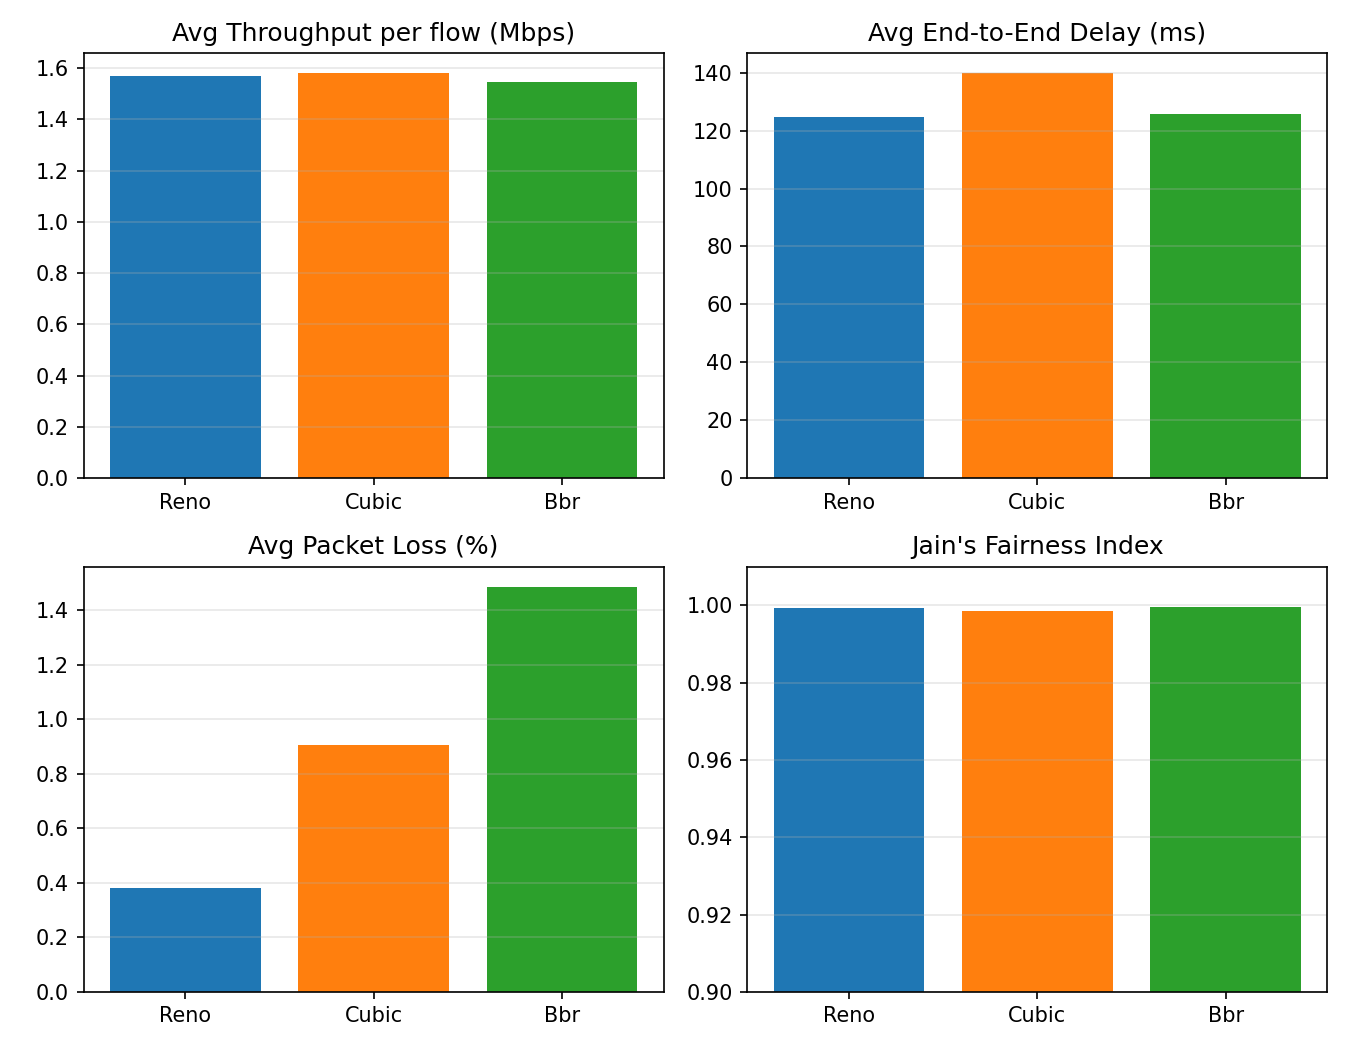
\includegraphics[width=0.85\textwidth]{screenshots/metrics_comparison.png}
\end{center}
\begin{center}
\renewcommand{\arraystretch}{1.2}
\begin{tabular}{lrrrr}
\toprule
\textbf{Variant} & \textbf{Avg Throughput (Mbps)} & \textbf{Avg Delay (ms)} & \textbf{Avg Loss \%} & \textbf{Fairness} \\
\midrule
Reno  & 1.570 & 124.6 & 0.38 & 0.9994 \\
Cubic & 1.581 & 139.8 & 0.91 & 0.9986 \\
BBR   & 1.547 & 125.8 & 1.49 & 0.9995 \\
\bottomrule
\end{tabular}
\end{center}

\section*{8. Comparison and Discussion}
\textbf{Throughput:} all three variants achieve nearly identical per-flow
throughput (~1.55--1.58~Mbps) because the 8~Mbps bottleneck shared by 5 flows
is the limiting factor here, not the congestion-control algorithm --
whichever algorithm is used, the link simply cannot deliver more.

\textbf{Delay:} Cubic produces the highest average delay (139.8~ms) because
its more aggressive window growth keeps the bottleneck queue fuller for
longer between loss events. Reno and BBR both settle closer to 125~ms.

\textbf{Packet loss:} Reno has the lowest loss (0.38\%) since it grows its
window the most conservatively. BBR has the highest loss (1.49\%) despite not
being loss-based itself -- it periodically probes for extra bandwidth
(its \texttt{PROBE\_BW} cycling) by briefly sending faster than the estimated
bottleneck rate, which causes short bursts of queue overflow.

\textbf{Fairness:} Jain's index is essentially 1.0 (0.9986--0.9995) for all
three algorithms. With five identical, saturating flows sharing one
bottleneck and no other asymmetry, none of the algorithms let one vehicle's
flow dominate the others.

\textbf{Why low delay and reliability matter for ITS:} a traffic-control
server acts on vehicle data to make time-critical decisions (e.g. adjusting
signal timing, issuing collision or road-hazard warnings). If that data
arrives late or is lost, the decision is made using stale information about
where vehicles actually are -- by the time a warning reaches a vehicle, the
hazard that triggered it may already have changed or passed, making the
warning useless or actively misleading. Unlike a file download, VANET safety
traffic has a very short useful lifetime, so low, predictable delay and
reliable delivery are the primary requirements, arguably more important than
raw throughput.

\section*{9. Learning Outcomes}
\begin{itemize}
  \item Built a multi-flow star/dumbbell topology in NS-3 to model several
        independent vehicles sharing one bottleneck path to a server.
  \item Selected between TCP Reno, Cubic, and BBR at runtime via
        \texttt{Config::SetDefault} on \texttt{TcpL4Protocol::SocketType},
        without changing the rest of the simulation.
  \item Traced a live TCP socket's congestion window using
        \texttt{Config::ConnectWithoutContextFailSafe} on a wildcarded
        attribute path, and visualised the resulting sawtooth/cubic/BBR
        shapes.
  \item Used \texttt{FlowMonitor} to compare throughput, delay, and loss
        across congestion-control algorithms, and computed Jain's Fairness
        Index to quantify how evenly flows shared the bottleneck.
  \item Understood, from the simulation results, why BBR's bandwidth-probing
        behaviour can cause more loss than classic loss-based algorithms even
        while achieving comparable throughput.
  \item Connected the measured delay/loss behaviour to a real requirement
        (VANET safety-data freshness) rather than treating the numbers as
        abstract.
\end{itemize}

\end{document}
